\documentclass[12pt,a4paper]{article}
% Estilo compartido para informes. Compilar con LuaLaTeX desde tp1/.
\usepackage[spanish,es-nodecimaldot]{babel}
\usepackage{fontspec}
\setmainfont{Montserrat-Medium.ttf}[
  Path=../assets/fonts/,
  BoldFont=Montserrat-Bold.ttf,
  ItalicFont=Montserrat-MediumItalic.ttf]
\usepackage[a4paper,margin=2.5cm,headheight=16pt]{geometry}
\usepackage{xcolor,graphicx,booktabs,tabularx}
\usepackage{float}
\usepackage{titlesec,fancyhdr,enumitem,caption}
\usepackage{ragged2e}
\usepackage{hyperref}
\definecolor{verde}{HTML}{1D4036}
\definecolor{bronce}{HTML}{D38129}
\definecolor{rosa}{HTML}{D88E77}
\definecolor{calido}{HTML}{EFE4D8}
\definecolor{grafito}{HTML}{1D1D1D}
\hypersetup{colorlinks=true,linkcolor=verde,urlcolor=verde,
  pdftitle={TP1 - Instalación de máquinas virtuales},pdfsubject={Cyberseguridad}}
\AtBeginDocument{\color{grafito}\RaggedRight\fontsize{12}{14.4}\selectfont}
\setlength{\parindent}{0pt}
\setlength{\parskip}{7pt}
\setlist[itemize]{leftmargin=*,itemsep=7pt,topsep=4pt}
\setlist[enumerate]{leftmargin=*,itemsep=6pt}
\titleformat{\section}{\color{verde}\bfseries\fontsize{18}{21.6}\selectfont}{\thesection}{0.65em}{}
\titleformat{\subsection}{\color{verde}\bfseries\large}{\thesubsection}{0.65em}{}
\titleformat{\subsubsection}{\color{verde}\bfseries}{\thesubsubsection}{0.65em}{}
\titlespacing*{\section}{0pt}{16pt}{8pt}
\titlespacing*{\subsection}{0pt}{12pt}{5pt}
\titlespacing*{\subsubsection}{0pt}{10pt}{4pt}
\setcounter{tocdepth}{2}
\pagestyle{fancy}
\fancyhf{}
\fancyhead[L]{\small\color{verde}FCEFyN | UNC}
\fancyhead[R]{\small\color{verde}\materia\ · TP \numeroTP}
\fancyfoot[L]{\scriptsize Informe de laboratorio}
\fancyfoot[R]{\small\thepage}
\renewcommand{\headrulewidth}{0.4pt}
\captionsetup{font=small,labelfont=bf,justification=raggedright,singlelinecheck=false,hypcap=false}
\newcommand{\pendiente}[1]{\par{\small\color{verde}\textbf{Por completar.} #1\par}}
% Si falta una captura se muestra un espacio reservado; no impide compilar.
\newcommand{\captura}[2]{%
  \par\smallskip\begingroup\centering
  \IfFileExists{figuras/#1}{%
    \includegraphics[width=\linewidth,height=5cm,keepaspectratio]{figuras/#1}%
  }{%
    \setlength{\fboxsep}{10pt}%
    \fcolorbox{bronce}{calido}{\parbox[c][1.25cm][c]{\dimexpr\linewidth-2\fboxsep-2\fboxrule\relax}{%
      \centering\small Captura pendiente\par\texttt{\detokenize{#1}}}}%
  }%
  \captionof{figure}{#2}\par\endgroup\smallskip
}

\usepackage{xurl}

\newcommand{\materia}{Cyberseguridad}
\newcommand{\numeroTP}{10}
\newcommand{\tituloTP}{Análisis de un ataque SQL}
\newcommand{\estudiante}{Brigido Tomas Andres}
\newcommand{\legajo}{38481096}
\newcommand{\carrera}{ICOMP}
\newcommand{\docente}{Javier A. Jorge}


% Metadatos específicos del TP10 y capturas en img/.
\hypersetup{pdftitle={TP10 - Análisis de un ataque SQL}}
\renewcommand{\captura}[2]{%
  \begin{figure}[H]
    \centering
    \IfFileExists{img/#1}{%
      \includegraphics[width=0.85\linewidth,height=5cm,keepaspectratio]{img/#1}%
    }{%
      \setlength{\fboxsep}{10pt}%
      \fcolorbox{bronce}{calido}{\parbox[c][1.1cm][c]{0.85\linewidth}{%
        \centering\small Captura pendiente\par\texttt{\detokenize{#1}}}}%
    }%
    \caption{#2}
  \end{figure}
}

\usepackage{caption}
\captionsetup{justification=centering}
\begin{document}
\hypersetup{pageanchor=false}
\begin{titlepage}
  
\includegraphics[width=8cm]{../assets/logo-fcefyn-2026.png}
  \vspace{1cm}

  {\color{verde}\small UNIVERSIDAD NACIONAL DE CÓRDOBA\par}
  \vspace{2.1cm}
  {\color{bronce}\bfseries\large TRABAJO PRÁCTICO \numeroTP\par}
  \vspace{0.45cm}
  {\color{verde}\bfseries\fontsize{32}{38.4}\selectfont Análisis de un\\ataque SQL\par}
  \vspace{0.3cm}
{\small Análisis de tráfico con Wireshark\par}
\vspace{0.35cm}
  {\large \materia\par}
  \vspace{0.8cm}
  {\color{bronce}\rule{2.7cm}{2pt}\par}
  \vfill
  \renewcommand{\arraystretch}{1.45}
  \begin{tabular}{@{}p{3.2cm}p{10cm}@{}}
    Estudiante & \estudiante \\
    Legajo & \legajo \\
    Carrera & \carrera \\
    Docente & \docente \\
  \end{tabular}
  \vfill
  {\small Córdoba, Argentina\par}
\end{titlepage}
\hypersetup{pageanchor=true}

\tableofcontents
\vspace{1cm}
\newpage

\section{Introducción y objetivos}
La actividad consiste en analizar una captura de un ataque de inyección SQL contra una aplicación que utiliza MySQL. Se seguirá la secuencia de solicitudes y respuestas HTTP para identificar la información obtenida y proponer medidas de prevención.

\section{Análisis del archivo PCAP}
\subsection{Paso 1: apertura de la captura}

\begin{figure}[H]
    \centering
    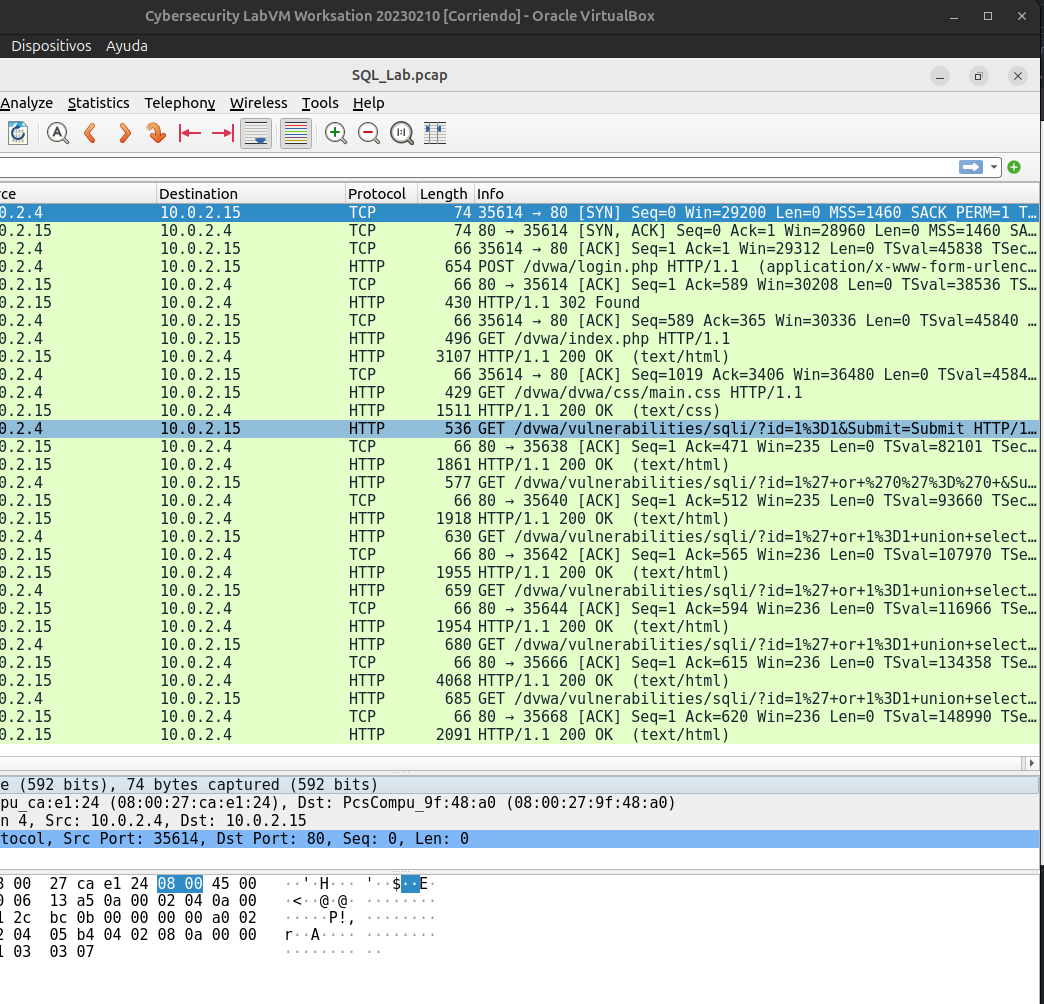
\includegraphics[width=0.9\textwidth]{img/captura.png}
    \caption{Primera vista de la captura de tráfico.}
    \label{fig:una-imagen}
\end{figure}

\par\textbf{¿ Cuáles son las dos direcciones IP involucradas en este ataque de inyección SQL ?}

Las dos ips involuradas son: 10.0.2.15 y 10.0.2.4

\subsection{Paso 2: comienzo del ataque}
Seguir el flujo HTTP del paquete 13 y buscar la cadena \texttt{1=1}, según la consigna.

\begin{figure}[H]
    \centering
    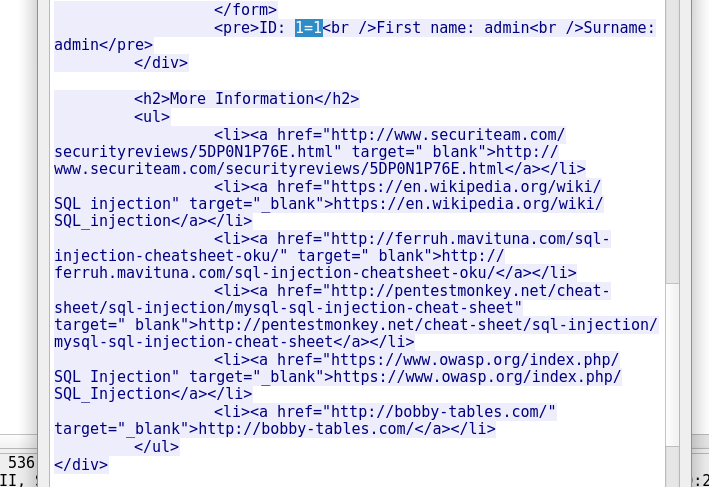
\includegraphics[width=0.9\textwidth]{img/1=1.png}
    \caption{Prueba de inyección SQL.}
    \label{fig:una-imagen}
\end{figure}

\subsection{Paso 3: identificación de la base de datos}
Seguir el flujo HTTP del paquete 19.

\begin{figure}[H]
    \centering
    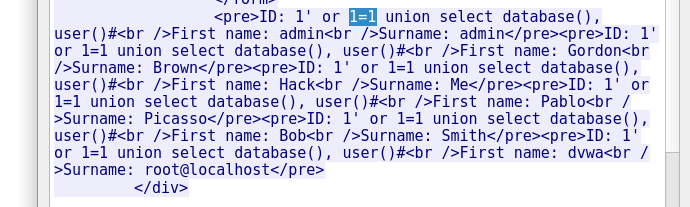
\includegraphics[width=0.9\textwidth]{img/segundo1=1.png}
    \caption{Prueba de inyección SQL con información de la base de datos.}
    \label{fig:una-imagen}
\end{figure}

\newpage
\subsection{Paso 4: información del sistema}
Seguir el flujo HTTP del paquete 22 y localizar el resultado de \texttt{version()}.

\begin{figure}[H]
    \centering
    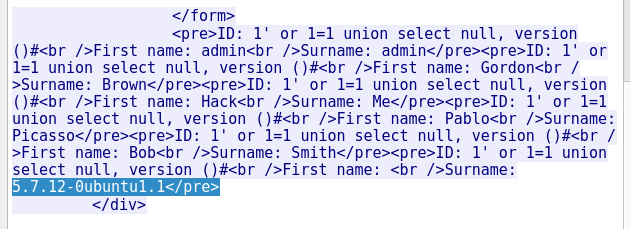
\includegraphics[width=0.9\textwidth]{img/version.png}
    \caption{Resultado de la función \texttt{version()}.}
    \label{fig:una-imagen}
\end{figure}

\par\textbf{¿ Cuál es la versión ?}
\texttt{5.7.12-0ubuntu1.1}

\subsection{Paso 5: información de tablas}
Seguir el flujo HTTP del paquete 25 y buscar \texttt{users}.

\begin{figure}[H]
    \centering
    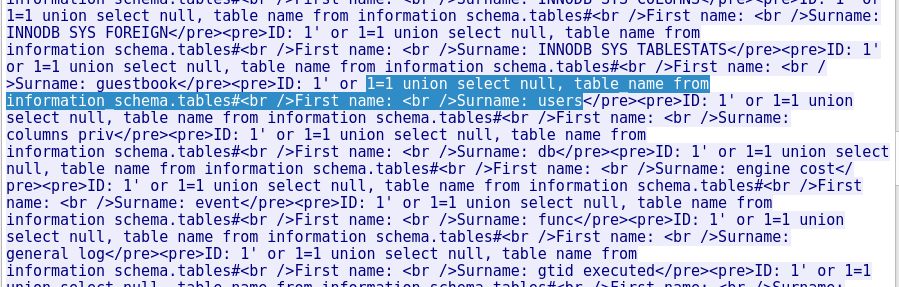
\includegraphics[width=0.9\textwidth]{img/pedidodetabla.png}
    \caption{Todas las tablas de la base de datos.}
    \label{fig:una-imagen}
\end{figure}

\par\textbf{¿ Qué haría el comando modificado ?}
\begin{verbatim}
1' OR 1=1 UNION SELECT null, column_name
FROM INFORMATION_SCHEMA.columns WHERE table_name='users'
\end{verbatim}

Permitiría al atacante conocer los nombres de las columnas de las tablas llamadas \texttt{users}, consultando \texttt{INFORMATION\_SCHEMA.columns}. Así podría identificar campos como \texttt{user} y \texttt{password} para preparar consultas posteriores, aunque esta consulta no devuelve sus valores.

\newpage
\subsection{Paso 6: usuarios y hashes de contraseñas}
Seguir el flujo HTTP del paquete 28.

\begin{figure}[H]
    \centering
    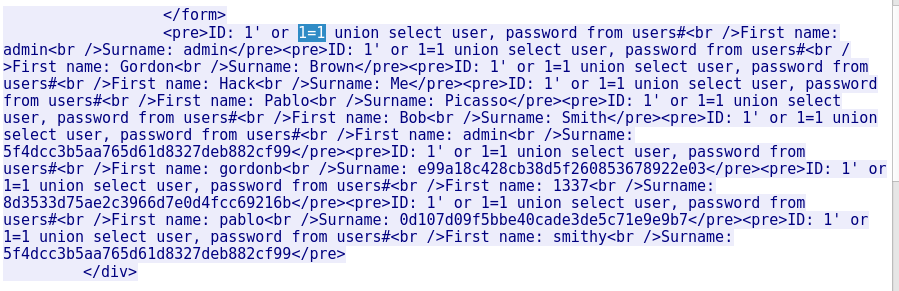
\includegraphics[width=0.9\textwidth]{img/contraseñas.png}
    \caption{Todas las contraseñas almacenadas.}
    \label{fig:una-imagen}
\end{figure}

\par\textbf{¿ Qué usuario tiene \texttt{8d3533d75ae2c3966d7e0d4fcc69216b} como hash de su contraseña ?}

\begin{figure}[H]
    \centering
    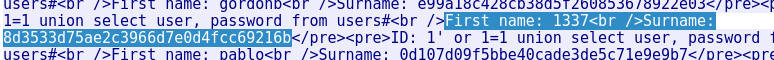
\includegraphics[width=0.9\textwidth]{img/hashpedida.png}
    \caption{Hash de ejemplo.}
    \label{fig:una-imagen}
\end{figure}

\begin{figure}[H]
    \centering
    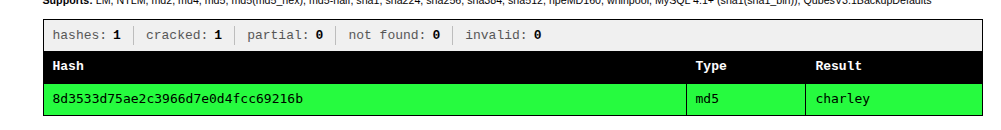
\includegraphics[width=\linewidth]{img/hash1decodificado.png}
    \caption{Hash 1 decodificado.}
    \label{fig:tres-primera}
\end{figure}

\begin{figure}[H]
    \centering
    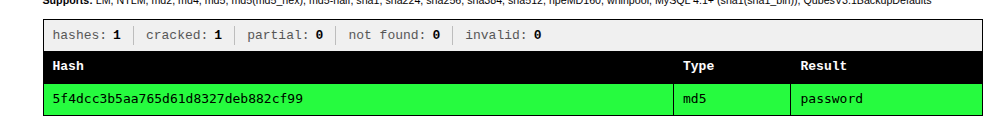
\includegraphics[width=\linewidth]{img/hash2decodificado.png}
    \caption{Hash 2 decodificado.}
    \label{fig:tres-segunda}
\end{figure}

\begin{figure}[H]
    \centering
    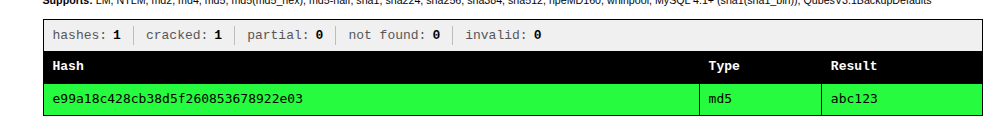
\includegraphics[width=\linewidth]{img/hash3decodificado.png}
    \caption{Hash 3 decodificado.}
    \label{fig:tres-tercera}
\end{figure}

\section{Entregable}
La inyección SQL ocurre cuando una aplicación interpreta entradas del usuario como parte del código de una consulta. Esto puede permitir consultar, modificar o eliminar datos sin autorización. El riesgo está en cómo se construyen las consultas, no en utilizar SQL.

\par\textbf{Métodos de ataque}
\begin{enumerate}
    \item \textbf{SQLi en banda:} utiliza el mismo canal para enviar la inyección y recibir información. Puede aprovechar mensajes de error o consultas con \texttt{UNION} para obtener datos en la respuesta de la aplicación, como en la captura analizada.
    \item \textbf{SQLi fuera de banda:} obtiene la información por un canal diferente, por ejemplo, mediante solicitudes DNS o HTTP hacia un servidor controlado por el atacante. Requiere que el entorno permita esas comunicaciones.
    \item \textbf{SQLi inferencial o ciega:} deduce información sin recibir directamente los datos de la base. El atacante observa cambios en las respuestas ante condiciones verdaderas o falsas, o diferencias en el tiempo de respuesta.
\end{enumerate}

\par\textbf{Métodos de prevención}
\begin{enumerate}
    \item \textbf{Consultas parametrizadas:} separan el código SQL de los valores ingresados por el usuario, de modo que estos se tratan como datos y no como instrucciones ejecutables.
    \item \textbf{Validación de entradas:} comprueba que los datos cumplan los tipos, formatos y valores permitidos por la aplicación. Complementa las consultas parametrizadas, pero no las reemplaza.
    \item \textbf{Mínimo privilegio:} limita los permisos de la cuenta utilizada por la aplicación a las operaciones necesarias. Esto reduce el alcance de los daños si se logra explotar una vulnerabilidad.
\end{enumerate}

\newpage
\section{Referencias}
Cisco Networking Academy. \textit{Práctica de laboratorio: Ataque a una base de datos mySQL}. Consigna local: \textit{7. Ataque DB a MySQL.pdf}.
\par CrackStation. \url{https://crackstation.net/}. Recurso indicado en la consigna.
\par Cloudflare. \href{https://www.cloudflare.com/es-es/learning/security/threats/how-to-prevent-sql-injection/}{Cómo prevenir la inyección SQL}.
\end{document}
